% Emission Curve Diagram
% Shows block reward decay with tail emission comparison to Bitcoin halvings
%
% ACCESSIBILITY ALT TEXT:
% A graph comparing emission schedules. X-axis shows years (0-20), Y-axis
% shows block reward. Botho's curve (blue, smooth) starts at 50 BTH and
% decays exponentially, reaching tail emission of 0.3 BTH which continues
% indefinitely. Bitcoin's curve (orange, stepped) shows discrete halvings
% every 4 years, eventually reaching zero. The smooth Botho curve avoids
% sudden supply shocks while ensuring perpetual security funding.

\begin{figure}[ht]
\centering
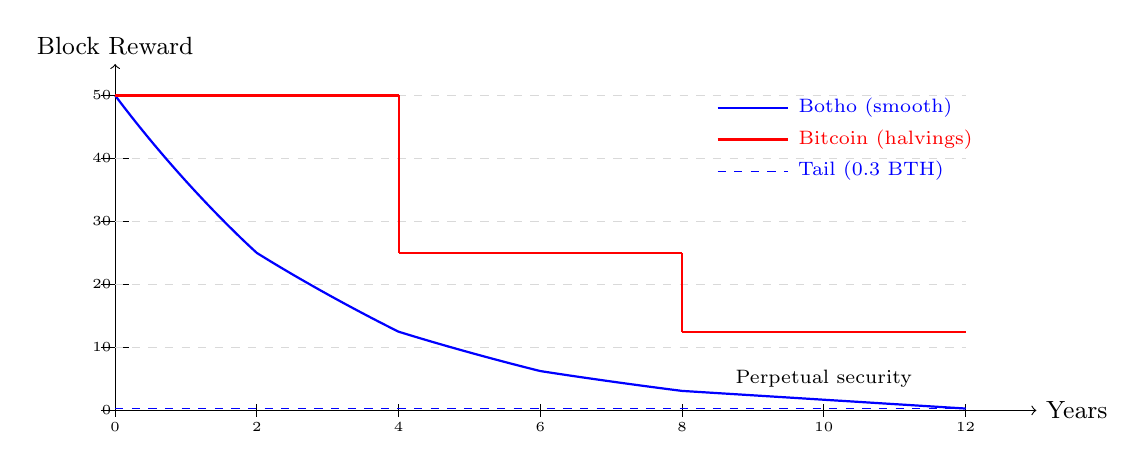
\begin{tikzpicture}[xscale=0.9, yscale=0.08]
    % Axes
    \draw[->] (0,0) -- (13,0) node[right] {\small Years};
    \draw[->] (0,0) -- (0,55) node[above] {\small Block Reward};

    % Y-axis labels
    \foreach \y in {0,10,20,30,40,50} {
        \draw (-0.2,\y) -- (0.2,\y) node[left=3pt] {\tiny \y};
    }

    % X-axis labels
    \foreach \x in {0,2,4,6,8,10,12} {
        \draw (\x,-1) -- (\x,1) node[below=3pt] {\tiny \x};
    }

    % Grid
    \draw[gray!30, dashed] (0,10) -- (12,10);
    \draw[gray!30, dashed] (0,20) -- (12,20);
    \draw[gray!30, dashed] (0,30) -- (12,30);
    \draw[gray!30, dashed] (0,40) -- (12,40);
    \draw[gray!30, dashed] (0,50) -- (12,50);

    % Botho smooth decay curve (approximated with line segments)
    \draw[blue, thick]
        (0,50) .. controls (1,35) and (2,25) .. (2,25)
        .. controls (3,18) and (4,12.5) .. (4,12.5)
        .. controls (5,9) and (6,6.25) .. (6,6.25)
        .. controls (7,4.5) and (8,3.1) .. (8,3.1)
        -- (12,0.3);

    % Bitcoin step function
    \draw[red, thick]
        (0,50) -- (4,50)
        (4,50) -- (4,25)
        (4,25) -- (8,25)
        (8,25) -- (8,12.5)
        (8,12.5) -- (12,12.5);

    % Tail emission line
    \draw[blue, dashed] (0,0.3) -- (12,0.3);

    % Legend
    \draw[blue, thick] (8.5,48) -- (9.5,48) node[right, font=\scriptsize] {Botho (smooth)};
    \draw[red, thick] (8.5,43) -- (9.5,43) node[right, font=\scriptsize] {Bitcoin (halvings)};
    \draw[blue, dashed] (8.5,38) -- (9.5,38) node[right, font=\scriptsize] {Tail (0.3 BTH)};

    % Annotation
    \node[font=\scriptsize] at (10,5) {Perpetual security};
\end{tikzpicture}
\caption{Block reward emission schedule. Botho uses smooth exponential decay
(halving every 2 years) transitioning to perpetual tail emission at 0.3 BTH,
compared to Bitcoin's discrete halving events. Tail emission ensures
long-term security funding.}
\label{fig:emission-curve}
\end{figure}
